% Gradopsy: a machine-learning engine written from scratch, and running in the browser.
%
% Build:   cd paper && python make_tables.py && latexmk -pdf main.tex
%          (or: pdflatex main && bibtex main && pdflatex main && pdflatex main)
% Every number in the experiments section is generated: the MNIST table by make_tables.py from the
% files the training script writes (demos/public/recognize/*.json), and the rest, with the figures,
% by experiments.ipynb. None is typed by hand.

\documentclass[11pt]{article}

\usepackage[a4paper, margin=2.6cm]{geometry}
\usepackage[T1]{fontenc}
\usepackage{lmodern}
\usepackage{microtype}
\usepackage{amsmath, amssymb, amsthm}
\usepackage{booktabs}
\usepackage{graphicx}
\usepackage{float}             % [H]: tables and figures stay where they are written
\usepackage{algorithm}
\usepackage{algpseudocode}
\usepackage{xcolor}
\usepackage{listings}
\usepackage[hidelinks]{hyperref}

\lstset{basicstyle=\ttfamily\small, columns=fullflexible, keepspaces=true, frame=none,
        xleftmargin=1.5em, showstringspaces=false}

\newcommand{\R}{\mathbb{R}}
\newcommand{\T}{^{\top}}
\newcommand{\dL}[1]{\frac{\partial L}{\partial #1}}  % the gradient of the loss with respect to #1
\newcommand{\code}[1]{\texttt{#1}}

\title{\textbf{Gradopsy}\\[2pt]\large A reverse-mode autodiff engine, its optimizers, and running it in the browser}
\author{Roberto Nsoni}
\date{\today}

\begin{document}
\maketitle

\begin{abstract}
Gradopsy is a small machine-learning engine written from scratch on top of NumPy: a tensor with
reverse-mode automatic differentiation, layers, losses, first-order optimizers (SGD, momentum,
RMSProp, Adam) and second-order ones (BFGS and damped Newton with a finite-difference Hessian)
under a strong-Wolfe line search. The same package runs unmodified in the browser through Pyodide,
where a website uses it to train and inspect networks live. This document derives every operation
and update rule exactly as implemented, describes how the implementation is verified, and reports
results on MNIST.
\end{abstract}

\section{Introduction}
\label{sec:intro}

Most people who train neural networks never see the machinery that makes it possible: the graph
that records every operation, the chain rule applied backwards through it, the update rule that
turns a gradient into a step. visualML is that machinery written out, small enough to be read in an
afternoon, and complete enough to reach the accuracy one expects on MNIST
(Section~\ref{sec:experiments}).

The project has two halves that share one codebase.
\begin{itemize}
  \item \textbf{The engine} (\code{src/visualml/}): a \code{Tensor} type with reverse-mode automatic
        differentiation (Section~\ref{sec:autodiff}), a set of differentiable operations
        (Section~\ref{sec:ops}), modules and losses (Section~\ref{sec:losses}), and six optimizers
        with a line search (Section~\ref{sec:optim}). It depends on nothing but NumPy.
  \item \textbf{The website} (\code{demos/}), which loads the same Python package into the browser
        with Pyodide (Section~\ref{sec:browser}) and uses it to train networks live, and to take a
        trained one apart number by number.
\end{itemize}

Two rules shape the code. Every differentiable operation is checked against a numerical gradient
before it is used (Section~\ref{sec:verification}). And nothing the website shows is reimplemented
in JavaScript: the page asks the engine, and draws what it answers.

The mathematics in this document is what the author learnt in the first two years of the
Bachelor's Degree in Data Science and Engineering (GCED) at the Universitat Polit\`ecnica de
Catalunya: linear algebra~\cite{upc-alg}, mathematical optimisation~\cite{upc-om}, machine
learning~\cite{upc-aa1} and audiovisual processing~\cite{upc-ipa}. The original papers and books
are cited where each method appears.

% TODO(author): one paragraph on motivation and on what you learnt building it.

\section{Tensor class}
\label{sec:autodiff}

\subsection{Definition}
A \code{Tensor} holds an array \code{data} (always \code{float64}), a flag \code{requires\_grad},
and, when the flag is set, three things about how it was made: the set of tensors it was computed
from (\code{\_prev}), a closure \code{\_backward}, and the name of the operation. Every operation
on tensors returns a new tensor, and if any input requires a gradient it records those three
fields. A forward pass therefore builds a directed acyclic graph whose leaves are the inputs and
the parameters, and whose root is, in training, the scalar loss $L$.

\subsection{The backward pass}
For a tensor $u$ in the graph, $\dL{u}$ is the gradient of the loss with respect to it: an array
with the same shape as $u$, stored in \code{u.grad}. If $v$ was computed from $u$ and $\dL{v}$ is
already known, the chain rule gives
\begin{equation}
  \frac{\partial L}{\partial u} = J\T\, \frac{\partial L}{\partial v},
  \qquad J = \frac{\partial v}{\partial u},
  \label{eq:chain}
\end{equation}
with $u$ and $v$ read as flat vectors and $J$ the Jacobian of $v$ with respect to $u$. This product
of a vector with the Jacobian is what each operation's \code{\_backward} computes for each of its
inputs, without ever building $J$: for an elementwise operation it is diagonal, and the product is
just another elementwise operation on arrays.

A tensor used by more than one operation receives a gradient from each, and by the chain rule they
add up. That is why every \code{\_backward} does \code{u.grad += \dots} and never \code{u.grad = \dots}.

\code{Tensor.backward()} first orders the graph topologically with an iterative depth-first
search, then sets $\partial L/\partial L = 1$ and calls \code{\_backward} on every node in reverse
topological order, so that each node's gradient is complete before it is passed on to its inputs.

\begin{algorithm}[H]
\caption{\code{Tensor.backward} (reverse mode)}
\begin{algorithmic}[1]
\State $\textit{order} \gets$ topological order of the graph reachable from $L$
\State \code{L.grad} $\gets 1$
\For{$v$ in reverse(\textit{order})}
  \State $v.\code{\_backward}()$ \Comment{adds its part of the gradient to the \code{.grad} of each input}
\EndFor
\end{algorithmic}
\end{algorithm}

Gradients are allocated lazily (as zeros, the first time they are read) and must be reset between
steps with \code{zero\_grad()}, which every optimizer does before evaluating the loss.

\subsection{Broadcasting}
NumPy broadcasting lets $a \in \R^{n\times m}$ be added to $b \in \R^{m}$. The forward is free; the
backward is not, because \code{b.grad} must have the shape of $b$. Since $b$ was copied along the
broadcast axes, its gradient is the sum of the incoming gradient over them. \code{reduce\_grad}
implements exactly this: it sums over the leading axes that broadcasting added, and over every axis
where $b$ had size $1$ but the result did not.

\subsection{Freezing a model}
A trained model used only for predictions does not need a graph: building one keeps every
intermediate array alive for a backward pass that never comes. \code{Module.freeze()} sets
\code{requires\_grad = False} on every parameter, after which a forward pass on a plain input
records nothing. A gradient with respect to an input that does require one is still computed
exactly, which is all that a saliency map needs.

\section{Operations}
\label{sec:ops}

Each operation is listed with its forward rule and the gradient it sends to each of its inputs,
following \eqref{eq:chain}, written on whole arrays. $a \ast b$ is the \emph{elementwise} product,
entry by entry (NumPy's \code{a * b}); $AB$, with nothing between the factors, is the matrix
product (\code{A @ B}); functions and powers of an array, such as $a^{p}$, $\beta^{a}$ or
$\tfrac{1}{a}$, act on each entry; and $[\,\text{condition}\,]$ is the array that is $1$ where the
condition holds and $0$ elsewhere (a boolean array used as numbers). When an input was broadcast,
its gradient is then summed over the broadcast axes by \code{reduce\_grad}
(Section~\ref{sec:autodiff}).

\subsection{Elementwise and linear algebra}
\begin{center}
\renewcommand{\arraystretch}{2.4}\renewcommand{\dL}[1]{\dfrac{\partial L}{\partial #1}}  % full-size fractions in the tables
\begin{tabular}{@{}lll@{}}
\toprule
operation & forward & gradient \\
\midrule
negation       & $v = -a$                  & $\dL{a} = -\dL{v}$ \\
addition       & $v = a + b$               & $\dL{a} = \dL{v}$,\ \ $\dL{b} = \dL{v}$ \\
product        & $v = a \ast b$            & $\dL{a} = \dL{v} \ast b$,\ \ $\dL{b} = \dL{v} \ast a$ \\
power ($p\in\mathbb{Z}$) & $v = a^{p}$     & $\dL{a} = \dL{v} \ast p\, a^{p-1}$ \\
exponential    & $v = \beta^{a}$           & $\dL{a} = \dL{v} \ast \beta^{a} \ln\beta$ \quad ($\beta = e$ by default) \\
logarithm      & $v = \log_\beta a$        & $\dL{a} = \dL{v} \ast \dfrac{1}{a \ln \beta}$ \\
sum            & $v = \sum_{\text{axes}} a$ & $\dL{a} = \dL{v}$ broadcast back to the shape of $a$ \\
mean           & $v = \tfrac{1}{N}\sum_{\text{axes}} a$ & $\dL{a} = \tfrac{1}{N}\, \dL{v}$ broadcast back \\
transpose      & $V = A\T$                 & $\dL{A} = (\dL{V})\T$ \\
reshape        & $V = \operatorname{reshape}(A)$ & $\dL{A} = \operatorname{reshape}(\dL{V}, \operatorname{shape}(A))$ \\
matrix product & $V = AB$                  & $\dL{A} = \dL{V}\, B\T$,\ \ $\dL{B} = A\T\, \dL{V}$ \\
\bottomrule
\end{tabular}
\end{center}
Subtraction and division are composed from these ($a - b = a + (-b)$, $a/b = a \ast b^{-1}$).
\code{sum} and \code{mean} keep the reduced axes (\code{keepdims}), which makes the broadcast back in
the backward pass exact; for \code{mean}, $N$ is the number of elements averaged.

\subsection{Activations}
\begin{center}
\renewcommand{\arraystretch}{2.4}\renewcommand{\dL}[1]{\dfrac{\partial L}{\partial #1}}  % full-size fractions in the tables
\begin{tabular}{@{}lll@{}}
\toprule
activation & forward & gradient \\
\midrule
ReLU    & $v = \max(0, a)$                 & $\dL{a} = \dL{v} \ast [\,a > 0\,]$ \\
sigmoid & $v = \sigma(a) = 1/(1 + e^{-a})$ & $\dL{a} = \dL{v} \ast v \ast (1 - v)$ \\
tanh    & $v = \tanh a$                    & $\dL{a} = \dL{v} \ast (1 - v^2)$ \\
\bottomrule
\end{tabular}
\end{center}
Sigmoid and tanh reuse their own output $v$ in the backward pass instead of recomputing it.

\subsection{Linear layers}
\code{Linear(n\_in, n\_out)} computes $Y = XW + b$ for a batch $X \in \R^{N\times n_\text{in}}$,
with $W \in \R^{n_\text{in}\times n_\text{out}}$ and $b \in \R^{n_\text{out}}$ broadcast over the
batch. It is composed of a matrix product and an addition, so its gradients come from the table
above; in particular $\dL{b_j} = \sum_{n} \dL{Y_{nj}}$, the sum over the batch that \code{reduce\_grad} does. Weights are
initialised as $W_{ij} \sim \mathcal{N}(0, 2/n_\text{in})$ (He initialisation~\cite{he2015}) and
biases as zero. \code{MLP}~\cite{upc-aa1} chains \code{Linear} layers with an activation between consecutive ones
and none after the last, which therefore outputs logits.

\subsection{Convolution}
\code{conv2d} takes $x \in \R^{N\times C\times H\times W}$, a filter bank
$w \in \R^{O\times C\times k_h\times k_w}$ and a bias $b \in \R^{O}$, stride $1$ and zero padding
$p$. With $\tilde x$ the padded input, it computes the cross-correlation (as every framework does,
under the name of convolution~\cite{upc-ipa})
\begin{equation}
  y_{n,o,i,j} = b_o + \sum_{c}\sum_{u=0}^{k_h-1}\sum_{v=0}^{k_w-1} w_{o,c,u,v}\,\tilde x_{n,c,i+u,j+v}.
\end{equation}
Rather than visiting every output position, the implementation loops over the $k_h k_w$ kernel
offsets $(u, v)$: for each, the shifted slice $\tilde x_{:,:,u:u+H_o,\,v:v+W_o}$ is contracted with
the $O\times C$ matrix $w_{:,:,u,v}$ over the channel axis (one \code{einsum}). The gradients are
\begin{align}
  \frac{\partial L}{\partial w_{o,c,u,v}} &= \sum_{n,i,j} \frac{\partial L}{\partial y_{n,o,i,j}}\,\tilde x_{n,c,i+u,j+v}, \\
  \frac{\partial L}{\partial \tilde x_{n,c,r,s}} &= \sum_{o}\sum_{u,v} \frac{\partial L}{\partial y_{n,o,r-u,s-v}}\, w_{o,c,u,v}, \\
  \frac{\partial L}{\partial b_o} &= \sum_{n,i,j} \frac{\partial L}{\partial y_{n,o,i,j}},
\end{align}
where the second sum only has the terms for which $(r-u, s-v)$ is a position of the output: an input
pixel receives a gradient from every output that used it. The code computes them with the same loop
over $(u, v)$ as the forward pass, adding each offset's share into \code{x.grad}, and finally cuts the
padding off.

\subsection{Max pooling}
\code{maxpool2d(k)} reshapes each $k\times k$ block of the input into its own axes and takes the
maximum over them, $y_{n,c,i,j} = \max_{0\le u,v<k} x_{n,c,ki+u,\,kj+v}$. Writing
$\operatorname{up}(\cdot)$ for repeating every value $k$ times along both spatial axes (so that it
covers its block again), the gradient is
\begin{equation}
  \frac{\partial L}{\partial x} = \operatorname{up}\!\Big(\frac{\partial L}{\partial y}\Big) \ast \big[\,x = \operatorname{up}(y)\,\big],
\end{equation}
which is exactly the code: \code{mask = x == y.repeat(k, 2).repeat(k, 3)}, times the gradient
repeated the same way. It flows only to the position that won each block. If two values of a block
tie for the maximum, both receive it; with real-valued inputs this has probability zero. A max-pool
has no parameters.

\section{Losses}
\label{sec:losses}

\subsection{Mean squared error}
$L = \frac{1}{N}\sum_{i} (\hat y_i - y_i)^2$, composed from subtraction, power and mean, so its
gradient follows from Section~\ref{sec:ops}.

\subsection{Cross-entropy from logits}
For logits $z \in \R^{N\times K}$ and integer labels $y \in \{0,\dots,K-1\}^N$, the softmax
$p_{ik} = e^{z_{ik}} / \sum_j e^{z_{ij}}$ and the cross-entropy~\cite{upc-aa1} are fused into one operation:
\begin{equation}
  L = \frac{1}{N}\sum_{i=1}^{N}\Big(-z_{i,y_i} + \log\sum_{j} e^{z_{ij}}\Big).
\end{equation}
The log-sum-exp is evaluated as $m_i + \log\sum_j e^{z_{ij} - m_i}$ with $m_i = \max_j z_{ij}$, which
leaves the value unchanged and keeps the exponentials from overflowing. Differentiating,
\begin{equation}
  \frac{\partial L}{\partial z_{ik}} = \frac{1}{N}\big(p_{ik} - Y_{ik}\big),
\end{equation}
where $Y_{ik}$ is $1$ if $k$ is the label of example $i$ and $0$ otherwise (the one-hot labels). So
the backward pass is the softmax minus the one-hot labels, divided by the batch size, without
ever building the softmax into the graph. This is both cheaper and numerically safer than composing
a softmax with a logarithm.

\subsection{Binary cross-entropy from logits}
For a single logit $z$ and a label $y\in\{0,1\}$, in the stable form
\begin{equation}
  L = \frac{1}{N}\sum_i \Big(\max(z_i, 0) - z_i y_i + \log\big(1 + e^{-|z_i|}\big)\Big),
  \qquad \frac{\partial L}{\partial z_i} = \frac{\sigma(z_i) - y_i}{N}.
\end{equation}

\section{Optimizers}
\label{sec:optim}

All optimizers act on the list of parameter tensors of a model. Write $x_k$ for all parameters
flattened into one vector and $g_k = \nabla f(x_k)$ for the gradient of the loss there, computed by
a \emph{closure} that zeroes the gradients, runs the forward pass and calls \code{backward()}.
The methods and their notation follow~\cite{upc-om, nocedal2006}.

\subsection{First order}
With learning rate $\alpha$:
\begin{align}
  \text{SGD:}\quad & x_{k+1} = x_k - \alpha g_k, \\
  \text{Momentum:}\quad & v_{k+1} = \beta v_k + g_k, \qquad x_{k+1} = x_k - \alpha v_{k+1}
                         \quad(\beta = 0.9), \\
  \text{RMSProp:}\quad & r_{k+1} = \rho r_k + (1-\rho) g_k^2, \qquad
                         x_{k+1} = x_k - \alpha \frac{g_k}{\sqrt{r_{k+1}} + \varepsilon}
                         \quad(\rho = 0.9,\ \varepsilon = 10^{-8}),
\end{align}
and Adam~\cite{kingma2015}, momentum and RMSProp together with bias correction:
\begin{equation}
\begin{gathered}
  m_k = \beta_1 m_{k-1} + (1-\beta_1) g_k, \qquad v_k = \beta_2 v_{k-1} + (1-\beta_2) g_k^2, \\
  \hat m_k = \frac{m_k}{1 - \beta_1^k}, \qquad \hat v_k = \frac{v_k}{1-\beta_2^k}, \qquad
  x_{k+1} = x_k - \alpha \frac{\hat m_k}{\sqrt{\hat v_k} + \varepsilon},
\end{gathered}
\end{equation}
with $\beta_1 = 0.9$, $\beta_2 = 0.999$, $\varepsilon = 10^{-8}$. Squares and square roots are
elementwise.

\paragraph{Learning-rate schedule.} \code{LinearDecay} decays the rate linearly from $\alpha_0$ to
$0.01\,\alpha_0$ over the first $k_{ld}$ steps and keeps it there:
$\alpha_k = (1 - k/k_{ld})\,\alpha_0 + (k/k_{ld})\, 0.01\,\alpha_0$ for $k \le k_{ld}$.

\subsection{Line search}
BFGS and Newton choose their step length $\alpha$ along a direction $d$ with a line search
satisfying the strong Wolfe conditions~\cite{nocedal2006}:
\begin{align}
  f(x + \alpha d) &\le f(x) + c_1 \alpha\, g(x)\T d, \tag{W1}\\
  |g(x + \alpha d)\T d| &\le c_2\, |g(x)\T d|. \tag{W2}
\end{align}
The implementation (\code{blsnw32}) follows Nocedal and Wright's Algorithms 3.5 and 3.6: a
bracketing phase that doubles $\alpha$ while $f$ keeps decreasing, then a zoom that shrinks the
bracket by bisection until both conditions hold. $c_1 = 10^{-4}$ throughout.

\subsection{BFGS}
BFGS keeps an approximation $H_k$ of the \emph{inverse} Hessian, starting from $H_0 = I$, and moves
along $d_k = -H_k g_k$. After a step $s_k = \alpha_k d_k$ with change in gradient
$y_k = g_{k+1} - g_k$, it updates
\begin{equation}
  H_{k+1} = (I - \rho_k s_k y_k\T)\, H_k\, (I - \rho_k y_k s_k\T) + \rho_k s_k s_k\T,
  \qquad \rho_k = \frac{1}{y_k\T s_k}.
\end{equation}
The Wolfe conditions guarantee $y_k\T s_k > 0$; near the minimum both $s_k$ and $y_k$ vanish and the
update is skipped when $y_k\T s_k \le 10^{-12}$. The first trial step of the line search is $1$, and
afterwards $\alpha_{\max} = 2(f_k - f_{k-1})/(g_k\T d_k)$ (falling back to $1$ if not positive).
Here $c_2 = 0.1$.

\subsection{Damped Newton}
Newton's method fits the local quadratic $m(p) = f + g\T p + \tfrac12 p\T (H + \lambda I) p$ and
moves to its minimiser, $d = -(H + \lambda I)^{-1} g$, the solution of a linear system~\cite{upc-alg}. The Hessian is approximated by forward finite
differences of the analytical gradient,
\begin{equation}
  H_{:,i} \approx \frac{g(x + h e_i) - g(x)}{h}, \qquad h = 10^{-5},
\end{equation}
and symmetrised as $(H + H\T)/2$, at a cost of $n+1$ gradient evaluations. The damping starts at
$\lambda = 10^{-3}$ and is multiplied by $10$ until $d$ is a descent direction ($d\T g < 0$), which
handles non-convex regions. The step length comes from the same line search with $c_2 = 0.9$.
Newton and BFGS are only practical for small models, and both require full-batch
gradients: minibatch noise destroys the curvature estimate.

\section{Verification}
\label{sec:verification}

\subsection{Gradient checking}
Every differentiable operation is tested against a numerical gradient before it is used. For a
tensor $t$ and a function $F$ whose output is summed to a scalar, each entry of the analytical
gradient is compared with the central difference
\begin{equation}
  \frac{\partial}{\partial t_i}\sum F(t) \approx \frac{\sum F(t + \epsilon e_i) - \sum F(t - \epsilon e_i)}{2\epsilon},
  \qquad \epsilon = 10^{-6},
\end{equation}
with an absolute tolerance of $10^{-6}$ ($10^{-5}$ for the full convolutional network). Inputs are
weighted by fixed random tensors before summing, so that every output position contributes
differently and a gradient routed to the wrong place cannot pass by symmetry. Besides each operation
on its own, the checks cover composite graphs (a shared sub-expression, a diamond), an MLP with
cross-entropy, and a complete convolutional network (convolution, ReLU, max-pool, reshape, linear,
cross-entropy) with respect to every parameter. The convolution is additionally compared with a
direct, loop-by-loop evaluation of its definition.

\subsection{Test inventory}
% TODO(author): regenerate this table if tests are added (pytest --collect-only -q).
\begin{center}
\begin{tabular}{@{}lr@{}}
\toprule
file & tests \\
\midrule
\code{test\_autograd.py} (gradient checks)         & 24 \\
\code{test\_tensor.py}                             & 20 \\
\code{test\_surfaces.py}                           & 14 \\
\code{test\_optim.py}                              & 13 \\
\code{test\_viz.py}                                & 11 \\
\code{test\_training.py}                           & 10 \\
\code{test\_module.py}                             & 8 \\
\code{test\_recorder.py}                           & 8 \\
\code{test\_loss.py}                               & 7 \\
\code{test\_linreg.py}                             & 6 \\
\code{test\_linesearch.py}                         & 5 \\
\code{test\_serialize.py}                          & 3 \\
\code{test\_data.py}                               & 1 \\
\midrule
total                                              & 130 \\
\bottomrule
\end{tabular}
\end{center}

Beyond gradients, linear regression trained with the engine converges to the closed-form
least-squares solution (tested, and measured for every optimizer in Section~\ref{sec:linreg}), and the
line search is tested against the Wolfe conditions it claims.

\section{Running in the browser}
\label{sec:browser}

The website is static: there is no server to train on. Instead, the engine itself runs in the
visitor's browser. Pyodide~\cite{pyodide} is CPython and NumPy compiled to WebAssembly; the page
downloads it once (about 15\,MB), installs the gradopsy wheel with \code{micropip}, and loads a
bridge module (\code{demos/src/engine.py}) that exposes a few functions to JavaScript. Nothing about
the mathematics is reimplemented in JavaScript: the page only sends inputs across and draws the
arrays that come back.

\paragraph{Identical numbers.} Running the same optimizer races and MLP training in native Python
and in Pyodide produces bit-identical results (measured in \code{demos/spike/}), which is expected:
both execute the same NumPy code on IEEE~754 doubles.

\paragraph{Speed.} Pyodide runs about $2.5$--$2.9\times$ slower than native for this workload; a
step of a small MLP takes about $2.4$\,ms, fast enough to train live inside animation frames. The
page advances training a few milliseconds per frame, so the tab never blocks.

\paragraph{What runs where.} The playground trains small MLPs live in the tab. The MNIST networks of
Section~\ref{sec:experiments} are trained offline with the same engine
(\code{scripts/train\_mnist.py}); the page loads their weights and computes every prediction,
saliency map and intermediate activation it shows with the engine, in the tab.

% TODO(author): a diagram of the bridge (page <-> engine.py <-> ml package).

\section{Experiments}
\label{sec:experiments}

Two experiments: a convex problem whose answer is known in closed form, to check that the
optimizers find it, and MNIST, to check that the engine trains real networks. The tables in this
section are written by \code{make\_tables.py} and by the notebook \code{paper/experiments.ipynb},
from files the code produced; none is typed by hand.

\subsection{Linear regression against the closed form}
\label{sec:linreg}

The data is $y = Xw + \varepsilon$, with $X \in \R^{200\times3}$ drawn from a standard normal,
$w$ drawn the same way and $\varepsilon \sim \mathcal{N}(0, 0.1^2)$. The model is a
\code{Linear(3, 1)} without bias trained on the MSE, and its answer is compared with the normal
equations, $w^* = (X\T X)^{-1} X\T y$. The Hessian of the loss is $\frac{2}{n}X\T X$, constant, so the
first-order methods use $\alpha = 1/L$ with $L$ its largest eigenvalue, the largest step that is
safe for a quadratic; Adam uses $\alpha = 0.05$. The second dataset is the same with the three
features multiplied by $1$, $10$ and $100$, which makes the problem badly conditioned.

\begin{table}[H]
\centering
\begin{tabular}{@{}lrrrr@{}}
\toprule
 & \multicolumn{2}{c}{well conditioned} & \multicolumn{2}{c}{scales 1, 10, 100} \\
\cmidrule(lr){2-3} \cmidrule(l){4-5}
optimizer & steps to $10^{-6}$ & final error & steps to $10^{-6}$ & final error \\
\midrule
SGD & 9 & 9.2e-16 & -- & 2.5e+00 \\
Momentum & 270 & 7.8e-12 & -- & 1.5e+00 \\
Adam & 286 & 2.0e-11 & 379 & 4.5e-09 \\
BFGS & 7 & 9.2e-10 & 8 & 2.4e-10 \\
Newton & 2 & 2.9e-13 & 2 & 1.3e-13 \\
\bottomrule
\end{tabular}
\caption{Linear regression with the engine against the normal equations: the number of steps until $\|w - w^*\| < 10^{-6}$ (-- if never, in 500 steps for the first-order methods and 30 for BFGS and Newton) and the distance at the end. Condition numbers 1.2 and 9310.}
\label{tab:linreg}
\end{table}


\begin{figure}[H]
\centering
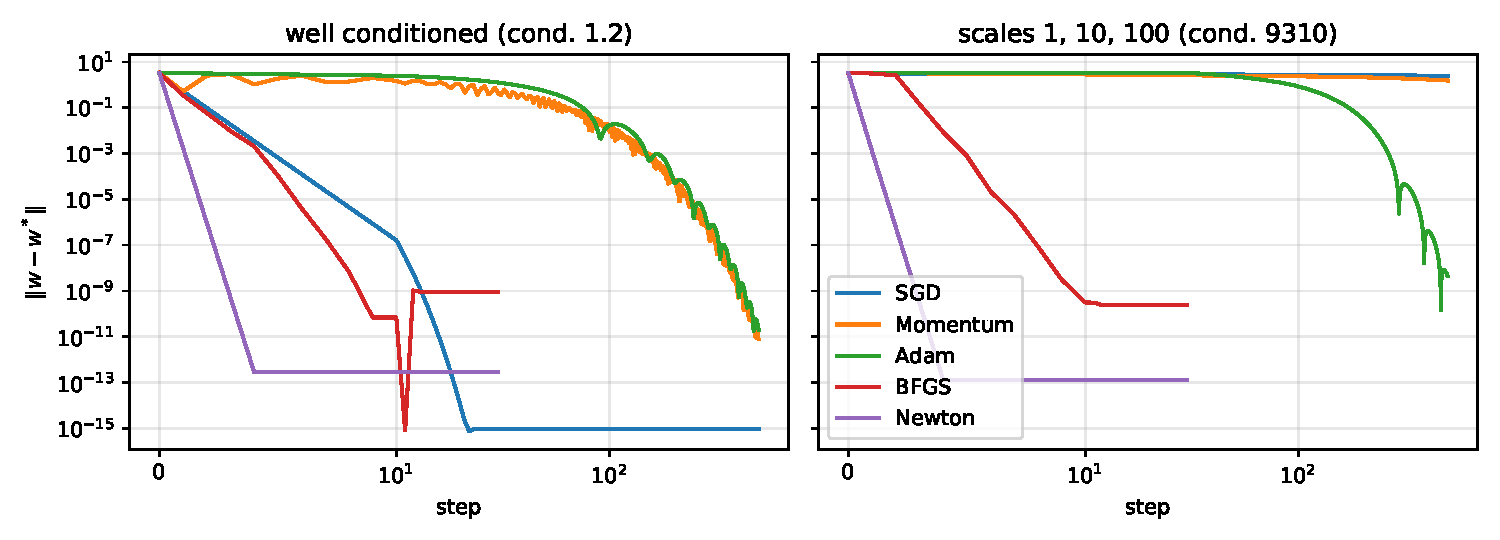
\includegraphics[width=\linewidth]{figures/linreg.pdf}
\caption{Distance to the closed-form solution at every step.}
\label{fig:linreg}
\end{figure}

With a condition number near 1 every method gets there, and plain gradient descent with
$\alpha = 1/L$ is among the fastest. With the features on different scales, the step that keeps the
steepest direction stable is far too small for the flattest one, and SGD and momentum are still
far from $w^*$ after 500 steps. Adam rescales every coordinate by its own gradient history, which
here largely undoes the scaling of the features. BFGS and Newton barely notice the conditioning:
damped Newton with a finite-difference Hessian is within $10^{-6}$ in a couple of steps on both
datasets, and BFGS needs a handful to learn the curvature.

% TODO(author): one or two sentences in your own words on what this says about first-order methods vs BFGS and Newton.

\subsection{MNIST}
\label{sec:mnist}

MNIST~\cite{lecun1998} has $60\,000$ training and $10\,000$ test images of $28\times28$ handwritten
digits. Pixels are scaled to $[0, 1]$. Two models, both trained with the engine:
\begin{itemize}
  \item \textbf{MLP}: $784 \to 256 \to 128 \to 10$, ReLU between layers.
  \item \textbf{CNN}: conv($1\to8$, $5\times5$, padding $2$), ReLU, max-pool $2\times2$,
        conv($8\to16$, $5\times5$, padding $2$), ReLU, max-pool $2\times2$, flatten, linear($784\to10$).
\end{itemize}
Both minimise the cross-entropy of Section~\ref{sec:losses} with Adam ($\alpha_0 = 10^{-3}$) on
minibatches of $64$, with the rate decaying linearly to $\alpha_0/100$ over the whole run
(\code{LinearDecay}). Every training minibatch is augmented: each digit is scaled by
$s \sim U(0.7, 1.3)$ about the centre and shifted by up to $13 - 10s$ pixels in each direction, so
that it stays inside the frame, by inverse mapping and bilinear interpolation~\cite{upc-ipa}; the
test set is not. The MLP is trained for 15 epochs and the CNN for 10. Each model is trained with
three seeds; test accuracy is measured once, at the end, on the float32 weights that are published
(the ones the website loads). The \emph{moved test} column is the same $10\,000$ test digits moved
and resized once in the same way, with a fixed seed.

\begin{table}[H]
\centering
\begin{tabular}{@{}lrrrlrr@{}}
\toprule
model & parameters & epochs & test accuracy (\%) & per seed & moved test (\%) & min / run \\
\midrule
MLP & 235,146 & 15 & $98.48 \pm 0.09$ & 98.49, 98.39, 98.56 & $97.38 \pm 0.02$ & 3.9 \\
CNN & 11,274 & 10 & $98.65 \pm 0.17$ & 98.85, 98.58, 98.53 & $97.49 \pm 0.20$ & 17.7 \\
\bottomrule
\end{tabular}
\caption{MNIST test accuracy, mean $\pm$ sample standard deviation over three seeds, on the test set as published and on the same digits moved and resized once with a fixed seed (moved test). Time is CPU training time in native Python.}
\label{tab:mnist}
\end{table}


The convolutional network is slightly more accurate with about $21\times$ fewer parameters: weight
sharing across positions builds in the translation structure that the MLP has to learn separately
for every pixel.

\begin{figure}[H]
\centering
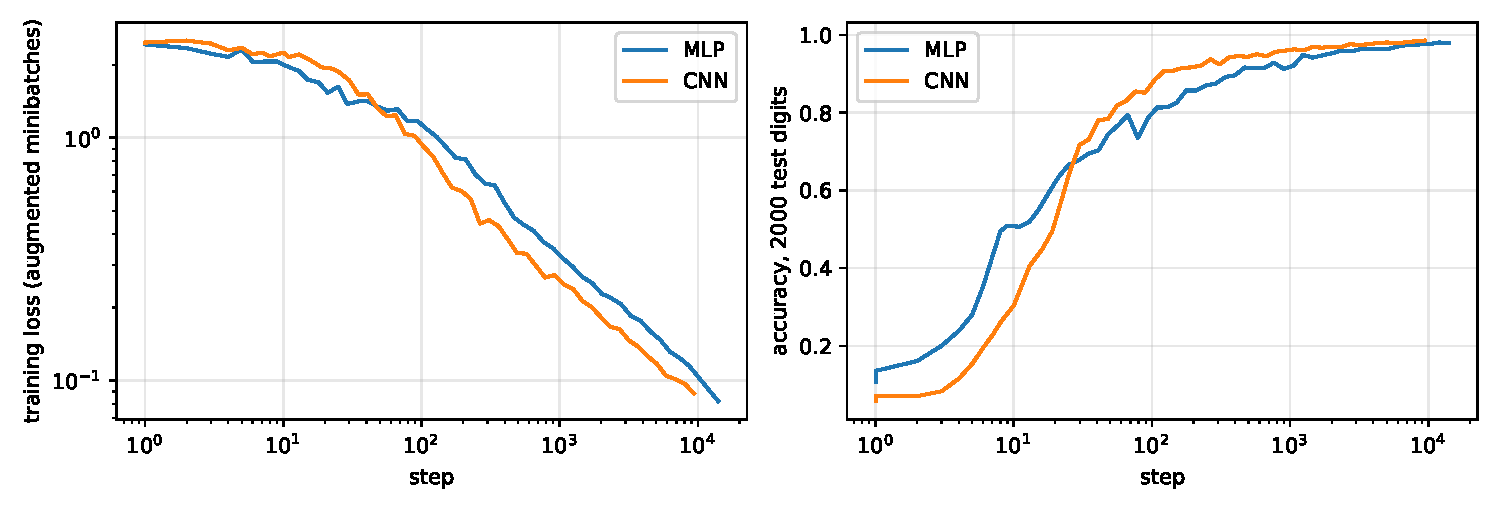
\includegraphics[width=\linewidth]{figures/mnist-curves.pdf}
\caption{Training loss (on the augmented minibatches) and accuracy on a fixed slice of $2\,000$ test
digits, at logarithmically spaced steps, for the published seed of each model.}
\label{fig:curves}
\end{figure}

Table~\ref{tab:shift} and Figure~\ref{fig:shift} give the test accuracy with every digit shifted
sideways, for the published models and for the same CNN trained without augmentation.

\begin{table}[H]
\centering
\begin{tabular}{@{}lrrrrrrrr@{}}
\toprule
 & \multicolumn{7}{c}{horizontal shift (pixels)} & \\
\cmidrule(lr){2-8}
model & $-6$ & $-4$ & $-2$ & $0$ & $+2$ & $+4$ & $+6$ & moved test \\
\midrule
CNN, no augmentation & 47.9 & 75.5 & 96.8 & 99.0 & 97.4 & 81.7 & 35.7 & 81.98 \\
CNN (published) & 93.2 & 97.5 & 98.4 & 98.9 & 98.5 & 97.2 & 88.9 & 97.72 \\
MLP (published) & 84.1 & 96.7 & 98.3 & 98.5 & 98.3 & 95.9 & 82.4 & 97.38 \\
\bottomrule
\end{tabular}
\caption{MNIST test accuracy (\%) with every digit moved sideways, and on the moved-and-resized test set of Table~\ref{tab:mnist}. The CNN without augmentation is the same network, seed and schedule as the published one, trained on the digits as they are; one seed.}
\label{tab:shift}
\end{table}


\begin{figure}[H]
\centering
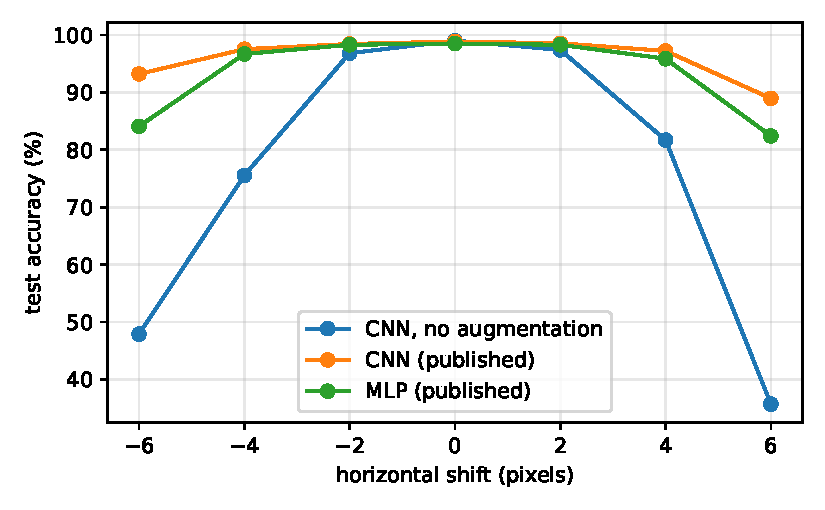
\includegraphics[width=0.6\linewidth]{figures/mnist-shift.pdf}
\caption{Test accuracy against a horizontal shift of every digit.}
\label{fig:shift}
\end{figure}

\section{Reproducibility}
\label{sec:reproducibility}

Everything in this document can be regenerated from the repository.
\begin{lstlisting}
pytest -q                                  # 130 tests, including every gradient check
python scripts/get_mnist.py                # MNIST into data/raw/mnist, md5-checked
python scripts/train_mnist.py --report     # both models x 3 seeds -> demos/public/recognize/
cd paper && python make_tables.py          # the MNIST table of section 8 from those files
jupyter nbconvert --to notebook --execute --inplace experiments.ipynb
                                           # linear regression, curves, shifts (~20 min)
latexmk -pdf main.tex
\end{lstlisting}
Training is deterministic given the seed. The published weights, the training logs and the
per-seed results are in \code{demos/public/recognize/}.


\bibliographystyle{plain}
\bibliography{refs}

\end{document}
